%%%%%%%%%%%%%%%%%%%%%%% file icad-template.tex %%%%%%%%%%%%%%%%%%%%%%
%% This is a template file for Springer Nature which is used for   %%
%% the International Conference of Axiomatic Design as of 2022     %%
%%                                                                 %%
%% Please do not use \input{...} to include other tex files.       %%
%% Submit your LaTeX manuscript as one .tex document.              %%
%%                                                                 %%
%% All additional figures and files should be attached             %%
%% separately and not embedded in the \TeX\ document itself.       %%
%%                                                                 %%
%% See sn-article for many more options to this template           %%
%%%%%%%%%%%%%%%%%%%%%%%%%%%%%%%%%%%%%%%%%%%%%%%%%%%%%%%%%%%%%%%%%%%%% 
\documentclass[sn-mathphys,pdflatex]{sn-jnl}% Math and Physical Sciences Reference Style

\jyear{2022}%

%% as per the requirement new theorem styles can be included as shown below
\theoremstyle{thmstyleone}%
\newtheorem{theorem}{Theorem}%  meant for continuous numbers
%%\newtheorem{theorem}{Theorem}[section]% meant for sectionwise numbers
%% optional argument [theorem] produces theorem numbering sequence instead of independent numbers for Proposition
\newtheorem{proposition}[theorem]{Proposition}% 
%%\newtheorem{proposition}{Proposition}% to get separate numbers for theorem and proposition etc.

\theoremstyle{thmstyletwo}%
\newtheorem{example}{Example}%
\newtheorem{remark}{Remark}%

\theoremstyle{thmstylethree}%
\newtheorem{definition}{Definition}%

\raggedbottom
%%\unnumbered% uncomment this for unnumbered level heads

%%Allow Icelandic characters
\usepackage[icelandic,english]{babel}
\usepackage[T1]{fontenc}

%% Setup graphics and paths
\usepackage{custom}
\usepackage{graphicx}
\graphicspath{{./}{Graphics/}}

%% packages to make tables look nicer
\usepackage{booktabs}
\usepackage{array} %% needed for advanced table manipulation
%% Column types from http://tex.stackexchange.com/questions/54069/table-with-text-wrapping
\newcolumntype{L}[1]{>{\raggedright\let\newline\\\arraybackslash\hspace{0pt}}m{#1}}
\newcolumntype{C}[1]{>{\centering\let\newline\\\arraybackslash\hspace{0pt}}m{#1}}
\newcolumntype{R}[1]{>{\raggedleft\let\newline\\\arraybackslash\hspace{0pt}}m{#1}}

\usepackage{url}%%URL should also be the last package loaded along with hyperref if needed

\begin{document}
\title[ICAD2022+ Template]{International Conference of Axiomatic Design 2022+ Template}

%%=============================================================%%
%% Prefix       -> \pfx{Dr}
%% GivenName    -> \fnm{Joergen W.}
%% Particle     -> \spfx{van der} -> surname prefix
%% FamilyName   -> \sur{Ploeg}
%% Suffix       -> \sfx{IV}
%% NatureName   -> \tanm{Poet Laureate} -> Title after name
%% Degrees      -> \dgr{MSc, PhD}
%% \author*[1,2]{\pfx{Dr} \fnm{Joergen W.} \spfx{van der} \sur{Ploeg} \sfx{IV} \tanm{Poet Laureate} 
%%                 \dgr{MSc, PhD}}\email{iauthor@gmail.com}
%%=============================================================%%


\author*[1,2]{\fnm{Joseph T.} \sur{Foley}}\email{foley AT ru.is}
\author[3]{\fnm{Erik} \sur{Puik}}
\author[4]{\fnm{Petra} \sur{Foith-Förster}}
\author[5]{\fnm{David S.} \sur{Cochran}}

\affil*[1]{\orgdiv{Department of Engineering}, \orgname{Reykjavik University}, \orgaddress{\street{Mennavegure 1}, \city{Reykjavík}, \postcode{102}, \country{Iceland}}}
\affil[2]{\orgdiv{Department of Mechanical Engineering}, \orgname{Massachusetts Institute of Technology}, \orgaddress{\street{77 Massachusetts Ave}, \city{Cambridge}, \postcode{02139}, \state{Massachusetts}, \country{USA}}}
\affil[2]{\orgname{Eindhoven University of Technology}, \orgaddress{\street{5612 AZ}, \city{Eindhoven}, \country{Netherlands}}}
\affil[2]{\orgdiv{Research Department}, \orgname{Bosch}, \orgaddress{\street{Robert-Bosch-Platz 1}, \city{Gerlingen}, \postcode{70839}, \country{Germany}}}
\affil[2]{\orgdiv{Department of Electrical Engineering}, \orgname{Purdue University Fort Wayne}, \orgaddress{\street{2101 East Coliseum Boulevard}, \city{Foprt Wayne}, \postcode{46805}, \state{Indiana}, \country{USA}}}

\abstract{All articles {\it must} contain an abstract.
The abstract serves both as a general introduction to the topic and as a brief, non-technical summary of the main results and their implications.
Authors are advised to check the author instructions for the journal they are submitting to for word limits and if structural elements like subheadings, citations, or equations are permitted.
Abtracts are often presented separately from the article, so they must stand on their own (no citations nor figure references).}

\keywords{keyword1, Keyword2, Keyword3, Keyword4}

\maketitle

\subsection*{Important Information}\label{sec:important-info}
This ICAD template is a customized version used in the SpringerNature book series ``Lecture Notes in Networks and Systems'' distributed at \url{https://www.springer.com/series/15179}.
The original SpringerNature \LaTeX{} template can be found at \url{https://www.springernature.com/gp/authors/campaigns/latex-author-support}
You will want to remove or comment out these sections before you begin adding your content.
Please read the \path{user-manual.pdf} before you begin writing your article:  it will save you a lot of hassle later.
If you want more detailed explanation of how to write things in the SpringerNature style, examine the \path{sn-article.tex}

\textbf{Important warning:  When using the SpringerNature's citation style called \path{sn-mathphys}, books {\em must\/} have an address field or you will get ``???'' showing up in the citation.
  Due to a bug in the current 2011 \path{sn-mathphys.bst} file, it won't give you an error or warning.}

  This template takes care of formatting and placement of the citations, as long as you fill in the BibTeX file \path{references.bib} and \path{references-ad.bib} correctly.
  If you are using crossrefs (to fill in the conference proceeding information), they must go at the end of the \path{.bib} file;  you can see examples of this near the end of \path{references-ad.bib}

  SpringerNature's submission system wants everything to be in the same directory.
  This means that you need to put the graphics and supplementary material in the directory with the main \verb|.tex| file or it will put blank spots where they would go.
  Joe recommends keeping everything in the Graphics folder until just before submission to keep everything clean or writing a script to flatten the directory structure when making your \verb|.zip| upload.
  
\subsection*{\LaTeX{} Hints}\label{sec:latex-hints}
\begin{itemize}
\item Rename this file to something unique with the year and topic like: \path{icad2022-sharklasers.tex} so you can find it more easily.
\item Put one sentence per line.
  This makes it easier to debug errors (which are by line) and to do grammar checking with \url{http://grammarly.com}.
\item Compile the document often and look for errors.
  If you find one, try commenting out the area to locate the source of the problem.
\item Watch out for \& and \%.  They have to have a left-slash in front of them.
\item Underscore ``\verb|_|'' is only usable in math as a subscript.
  Don't put it in normal text.
\end{itemize}


\section{Introduction}\label{sec:introduction}
The Introduction section expands on the background of the work (some overlap with the Abstract is acceptable).
The introduction should not include subheadings.

What is the idea?  What is it called and why?
Who is the target customer?



\subsection{Customer Needs}\label{sec:customer-needs}
What would a customer need the item to do?  
Using Axiomatic Design theory, this is stated as a numbered list of Customer Needs(CN)~\cite{suh1990principles}.
The top level is \CN0.
This is often (but not always) decomposed into \CN1, \CN2, etc.
Here is an example of a top level:

\begin{quote} \textbf{\CN0} A transfer bin for whole salmon, compatible with the SureTrack grader, cheaper and less prone to cracking due to skewing.  
The bin should be adaptable to a pure transfer task and be able to discharge anywhere along its path without
accidental discharge.~\cite{gerhard2016suretrack}
\end{quote}


\section{Prior Art}\label{sec:prior-art}
What exists that is similar?  How is yours better/distinctive?
Give at least two examples and quantify the differences (numeric values).
If you say something is cheaper, you need to give the costs for both items.

An example of a figure is the four Axiomatic Design domains in Fig.~\ref{fig:ad-domains}.
\begin{figure}
  \centering
  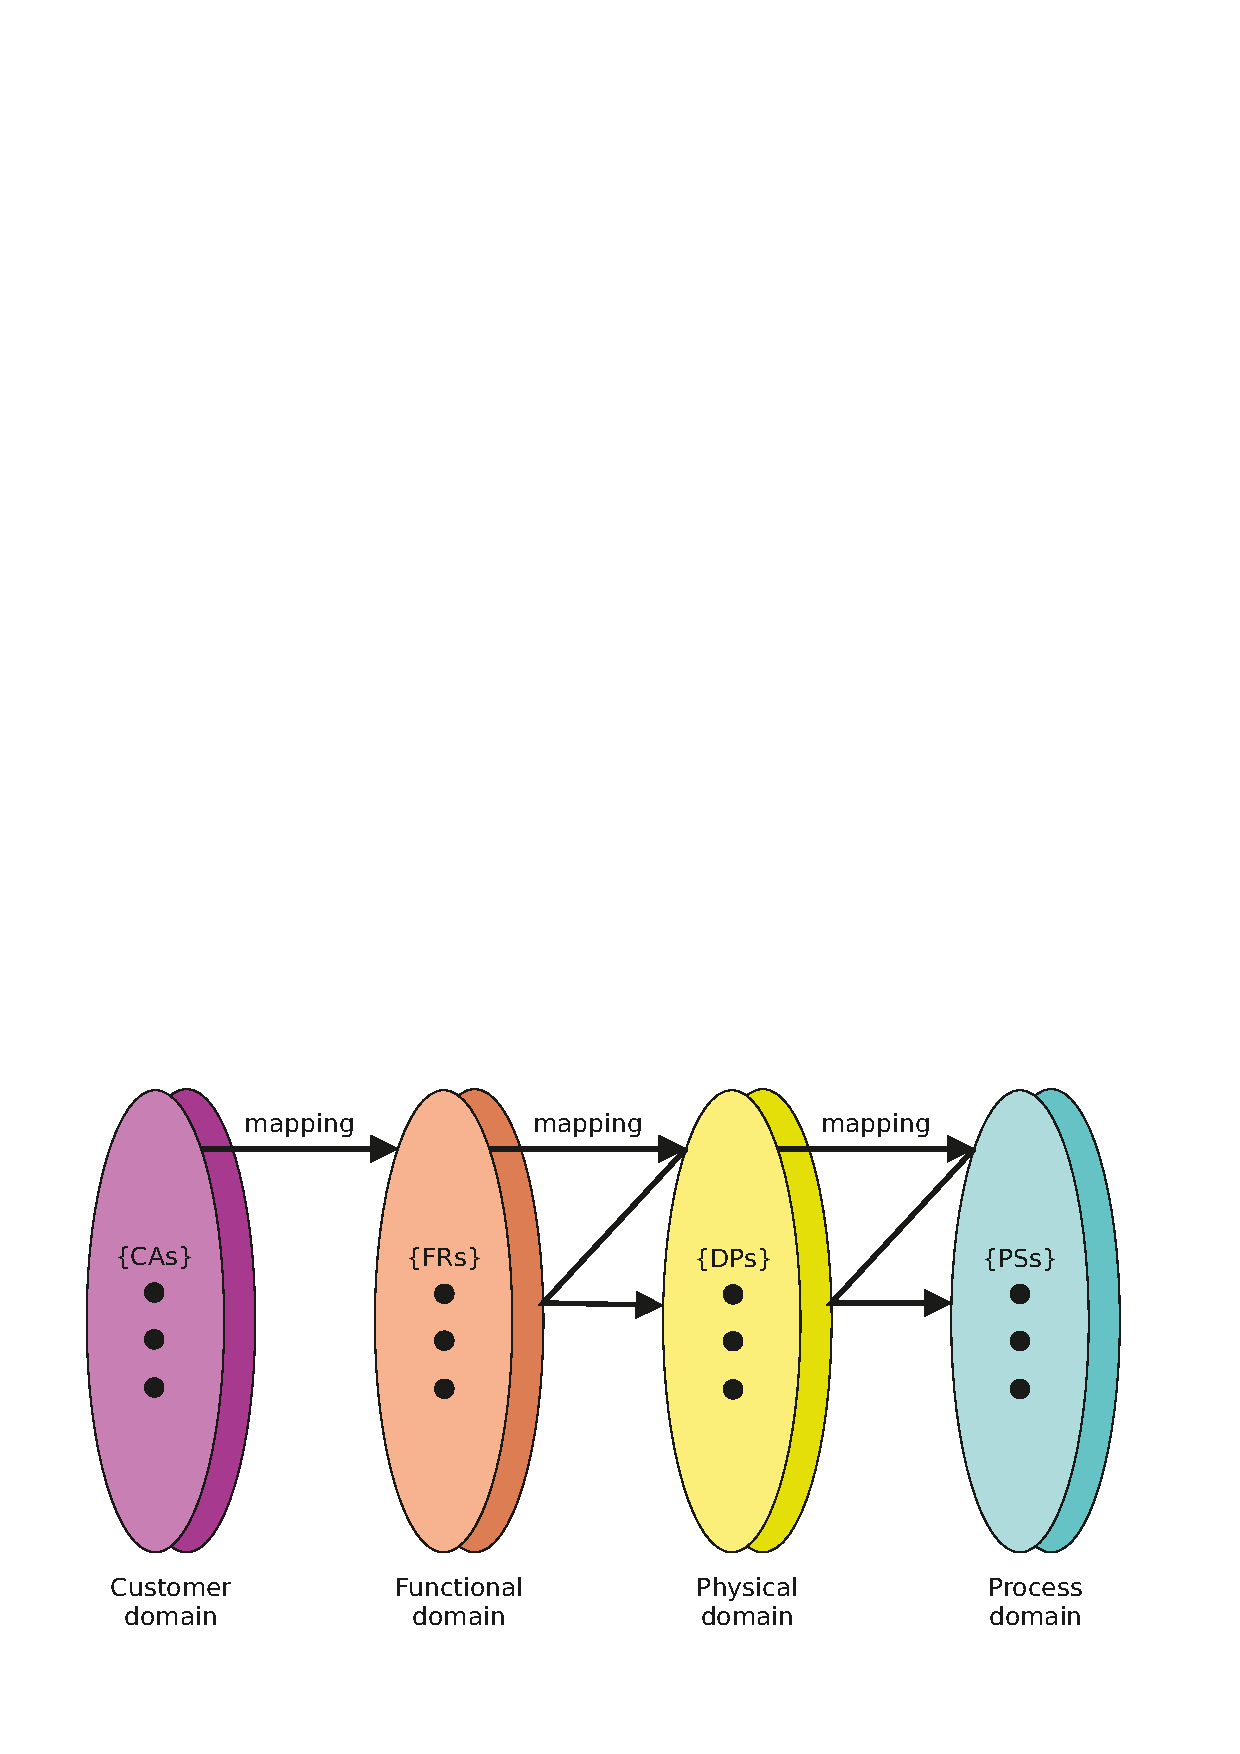
\includegraphics[width=0.9\columnwidth]{ad-domains-zig}
  \caption{General progression between the Axiomatic Design domains employing the zig-zag approach}\label{fig:ad-domains}
\end{figure}



\subsection{Sources}\label{sec:sources}
You will want to cite all these similar concepts/products.
As an example of a citation, Carryer et al.~\cite{carryer2011IntroMechatronics} is the textbook for T-411-MECH Mechatronics 1.


\section{Design}\label{sec:design}
As previously mentioned, using Axiomatic Design Theory is a good way to develop your design.

Here is a brief synopsis from Omarsdóttir et al.\cite{omarsdottir2016chessmate}:
\begin{quotation}
  Rather, the focus was placed on developing comprehensive FR and DP lists, then evaluating the coupling between them.
  This coupling is symbolized in a design matrix, which is a Cartesian product of all FR and DP combinations~\cite{cochran2016msdd, benevides2012aed}.
Where there is an interaction between an FR and DP, this is denoted by a non-zero coefficient, or in the case of the value being unknown, simply a placeholder variable $X$.
Minor levels of coupling, often considered higher-order effects, are annotated with $x$ to show their lessened effect.
A diagonal matrix is ``uncoupled'' and satisfies the Independence Axiom: ``to maintain the independence of the functional requirements~(FRs)''~\cite{suh2001axiomatic}.
Such a design can be easily optimized by adjusting a particular FR or DPs without affecting others.
A diagonal matrix indicates a ``decoupled'' or ``path-dependent'' solution, which can still be optimized, but the ordering of parameter choice selection becomes important.
All other design matrices are ``coupled'' and may have a usable local solution but usually resist modification and optimization~\cite{suh2001axiomatic}.
Needless to say, the focus is on minimizing coupling wherever it may appear.

ADT's second axiom is ``minimize the information content of the design.''
Simply put, ensure that the design has the highest probability of meeting the stated FRs.
When systems are not able to meet FRs all of the time, this is denoted in ADT as ``complexity'' and is deeply explored in~\cite{suh2005complexity}.
As will become apparent in the next section, this axiom became integral to the design of the interaction between the robot and its chess pieces.
Finally, any factors to be considered that are not functional are categorized as ``Constraints.''
These are often resource-focused and affect all of the design decisions; they need to be revisited often especially when choosing between otherwise equivalent implementations.
\end{quotation}
The first axiom is often called the Independence Axiom, and the second, the Information Axiom.


From the Customer Needs, we build a list of Functional Requirements.

Again, we start with a top-level \FR0: ``Contain \SI{25}{\kilogram} of fish on SureTrack conveyor until release is triggered''
From this, a top-level Design Parameter \DP0: Gable-reinforced stainless-steel locking bin with bi-directional discharge
\cite{gerhard2016suretrack}.

We continue a ``zig-zag'' procedure to decompose and map the FRs to the DPs as shown in Table~\ref{tab:first_level-frdp}.

\begin{table}
  \center
  \caption{First level FR-DP mapping.~\cite{gerhard2016suretrack}}\label{tab:first_level-frdp}
  \begin{tabular}{lll} \toprule
    ID& Functional Requirement & Design Parameter \\ \midrule 
    1&Contain product&Main weldment\\
    2&Move product&Support system\\
    3&Discharge product &Discharge system\\
    \bottomrule
  \end{tabular}
\end{table}

From this mapping we develop a design matrix as shown in Equation~\ref{eq:top-design-matrix} from~\cite{gerhard2016suretrack}.

\begin{equation}\label{eq:top-design-matrix}
\begin{Bmatrix}
\FR{1}\\
\FR{2}\\
\FR{3}
\end{Bmatrix}=
\begin{bmatrix}
X &  0 & X\\
0 &  X & 0\\
0 &  0 & X
\end{bmatrix}
\begin{Bmatrix}
\DP{1}\\
\DP{2}\\
\DP{3}
\end{Bmatrix}
\end{equation}

This matrix is de-coupled i.e.\ path-dependent, meaning it can be optimized, but the order matters.

\section{Results/Experiments/Prototypes}\label{sec:rep}

\section{Discussion}\label{sec:results-discussion}

\section{Conclusion}\label{sec:conclusion}

\subsection{Future work}\label{sec:future-work}

\subsection{Summary}\label{sec:summary}

\section*{References}\label{sec:references}
%\bibliographystyle{sn-mathphys}%%NOT NEEDED:Class file sets the style
\bibliography{references,references-ad}


\end{document}



%%% Local Variables:
%%% mode: latex
%%% TeX-master: t
%%% End:
